%!TEX root = project.tex

\chapter{Methodology}

For the project we used the waterfall methodology. We started by mapping out the requirements for the project. Then we designed how the UI would be implemented, how the user should be able to add an account on the system.  We used GitHub for source control of the program, we also used overleaf for collaboration with the dissertation.

We had regular meetings as a group and also with the group supervisor to discuss issues we were facing with the project and to make any changes that needed to be made.

\section{Requirements}

We mapped out the requirements of our project:
\begin{itemize}
\item We would need a server or some form of central point that connects the users to any back-end that we \item would require too run the game.
\item We decided the system required a login system that would allow a user to create an account or login to an existing one.
\item We then would need a system that allowed players to connect to other users.
\item We would need a lobby systems where players can wait for a game to start or wait for other players to join the game.
\item Once the game has ended we would need a system that could keep track of the players games and achievements such as a scoreboard system.
\item The separate systems speak to the client and do not need to send data to each other, this will allow the system to be interchangeable.
\item Element of the system should be capable of being replaced by another system, without replacing other parts of the system. For example, if we decided to change the database or language for the scoreboard system, we should be able to do so without having to change any part of the login system, the match making system and minimal changes to the game itself, if any.
\end{itemize}


The game Itself:
\begin{itemize}
\item Must have a procedural track to allow for non repetitive play.
\item Different versions of the game should connect to any instance and should not need to specify whether they can play with desktop or virtual reality headset users.
\item Desktop platforms must be able to see head and hand movement from the head mount display players.
\item Players must start in specified positions and must not have to enter any input for this to occur.
\item The Races must have a start and end point.
\end{itemize}

\newpage
\section{Design Stage}

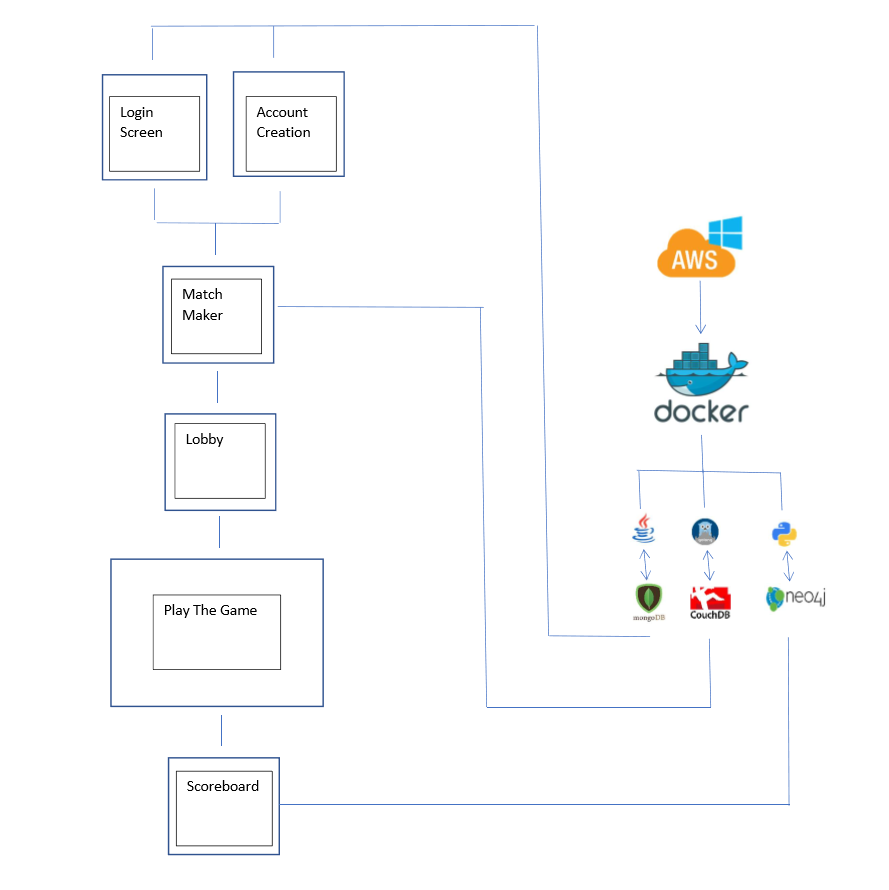
\includegraphics[width=1\columnwidth]{img/Overview.PNG}
\subsection {Overview}
The design stage is a critical and vital part of a software development project. Without first setting out goals and deliverables, a project can quickly lose it way. Design and modelling have been used in various projects dating back to the Ancient Egyptians and Romans and has been used many civilisations since. This process is widely used in science and engineering to give a high-level view of the system.
The first stage is to create a design document and a model of the intended project. This document is a detailed layout of the system used to give an overall guide to the architecture of the project. It should include attributes and relationships between data and their structures along with architectural, interface and procedural designs.

The next stage is to design a model of the project. This model is then used to obtain a better understanding of the system and is referenced to help understand the flow of data the various steps that take place throughout the project. 

The next stage of design is the analysis stage. This part of the process is about analysing the performance of the various stages of the software and its requirement and limitations. This is a vital part of the process and extremely relevant to our project as there was many different technologies and programming languages used. With these factors researched and discussed, we began the task of designing our project.

\subsection {The Game}
During the design stage, we had to map out the system and decide on which elements were needed and how they could be implemented. From the very start we knew that the game itself must be implemented in either Unity with C\# or using the Unreal 4 engine with C++. Our knowledge and experience of the unreal engine and with any of the C\p\p language is very limited, were as we already have a working knowledge of unity and C\#. So we went with Unity. Using any form of third gaming engine would not be practical as the libraries for the virtual reality devices have been focuses on these two implementations.\newline

\subsection {System Back-end}
We then needed to consider the back-end of the system and which platform were available. Firstly we could have used a physical computer that we personally owned and set it up as a running server. This would not have been a bad idea as we already own personal computers that could have effectively done this. Other options included using cloud based servers such as Amazon Web Services(AWS) or Google cloud. We had setup some instances of google cloud, we even ran them and began launching some of the programs on the system. From prior experiences, we had encountered situations were we had been charged by google cloud for use of such cloud instances and had found(AWS) to be a much cheaper rate. We also had some prior experience with AWS and opening firewall rules for this service, as we are using sockets, this was certainly going to be needed.\newline

\subsection {Login system}\newline
Development of the login system started with creating two java programs that used sockets to make a connection to one another. A socket is one endpoint of two-way communication between two programs running on a network with a corresponding socket on the other end. Each socket is bound to a port number that the TCP layer can identify that allows data to be sent back and forth between the two programs.\newline

Before development went any further a decision was made to use MongoDB as our database for the user login. The installation of MongoDB involved logging into the AWS virtual machine we are using for our project. For this project we decided to use the free version of MongoDB known as the community version using the current stable release (4.0.3) (MSI).\newline

To install mongo:\newline
•	Click on the file just downloaded which opens the installer.\newline
•	Click Next.\newline
•	Accept Terms & Conditions and click Next.\newline
•	Choose Complete Setup.\newline
•	Click Install.\newline
•	Click Finish.\newline


our login system

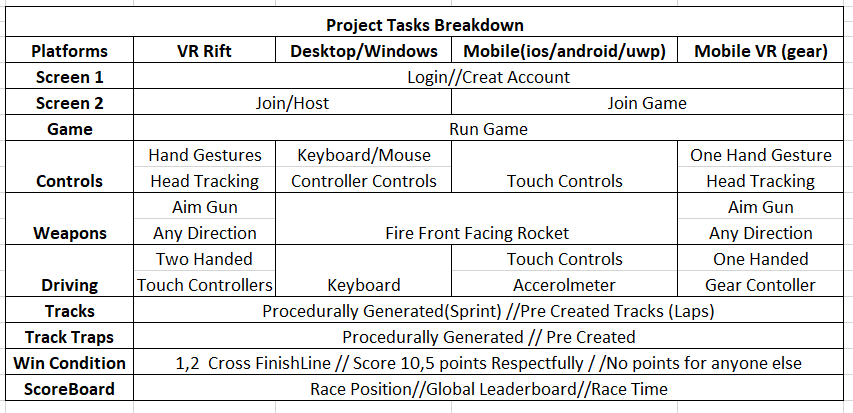
\includegraphics[width=1\columnwidth]{img/breakdown.PNG}

Our match making system

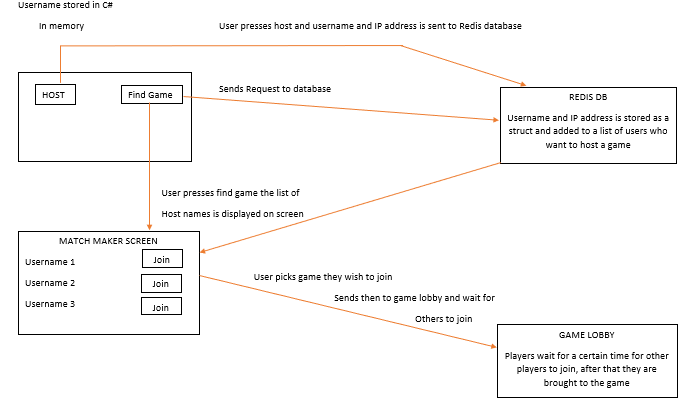
\includegraphics[width=1\columnwidth]{img/redisMatch.PNG}

An overview of the game

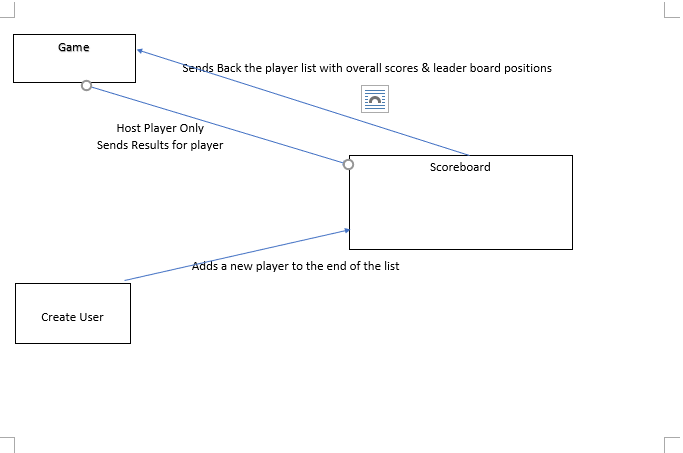
\includegraphics[width=1\columnwidth]{img/MariaDBPic.PNG}

An overview of our scoreboard system

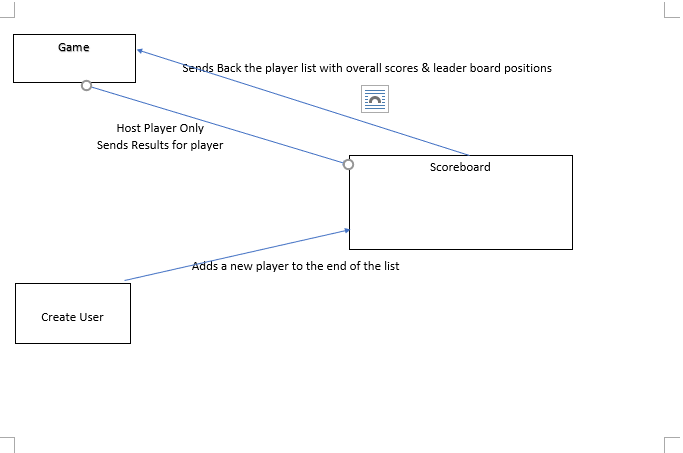
\includegraphics[width=1\columnwidth]{img/MariaDBPic.PNG}

\newpage
\section{Implementation}

\newpage
\section{Integration and System Testing}